% Created 2024-12-18 Wed 14:29
% Intended LaTeX compiler: pdflatex
\documentclass[presentation, smaller, aspectratio=169]{beamer}
\usepackage{graphicx}
\usepackage{float}
\usepackage{minted}
\author{Richard Graham, Martin Richter}
\date{19/12/2024}
\title{Version Control Training}
\subtitle{An Introduction to Git}
\begin{document}

\maketitle
\begin{frame}[label={sec:org540ed3e}]{Schedule}
\begin{center}
\begin{tabular}{rrl}
10:00 &  & Arrival and introduction\\
\hline
10:30 &  & Introduction to git\\
 & 10:30 & Creating a new repository\\
 & 10:50 & Changing files, view history\\
 & 11:10 & Creating branches\\
 & 11:30 & Showing differences\\
 & 11:50 & Merging branches\\
 & 12:10 & Aborting a merge\\
 & 12:30 & Merge conflicts\\
\hline
13:00 &  & Lunch\\
\hline
14:15 &  & Resolving a conflict in real\\
\hline
15:00 &  & Making it all work together\\
 &  & (Unit tests, refactoring)\\
\hline
16:00 &  & Close\\
\hline
\end{tabular}
\end{center}
\end{frame}
\begin{frame}[label={sec:org97707ef}]{Version Control: Reasons to Use It}
\begin{itemize}
\item What is Version Control?

A method to track changes as you develop code

\item \ldots{} and why to use it?
\end{itemize}
\end{frame}
\begin{frame}[label={sec:org6aabc51}]{Branching Example: Writing Paper (Draft)}
\begin{center}
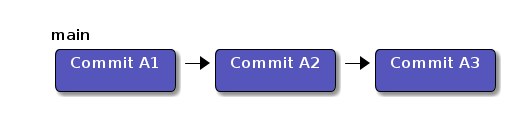
\includegraphics[scale=0.3]{figures/main_branch_010.png}
\label{branching_010_paper_draft}
\end{center}
\end{frame}
\begin{frame}[label={sec:orgcbbc9e3}]{Branching Example: Submit Paper}
\begin{center}
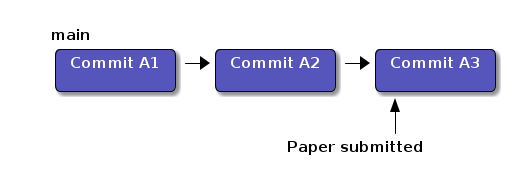
\includegraphics[scale=0.3]{figures/main_branch_020.png}
\label{branching_020_submit_paper}
\end{center}
\end{frame}
\begin{frame}[label={sec:orgd4ab1fb}]{Branching Example: New Idea!}
\begin{center}
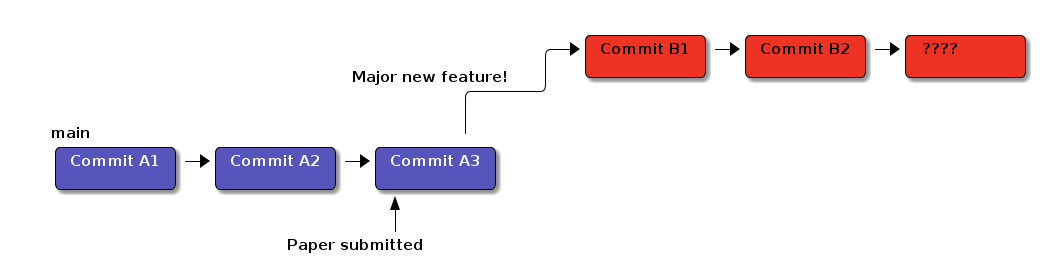
\includegraphics[scale=0.3]{figures/main_branch_030.png}
\label{branching_30_develop_new_idea}
\end{center}
\end{frame}
\begin{frame}[label={sec:org91a9870}]{Branching Example: Referee Changes!}
\begin{center}
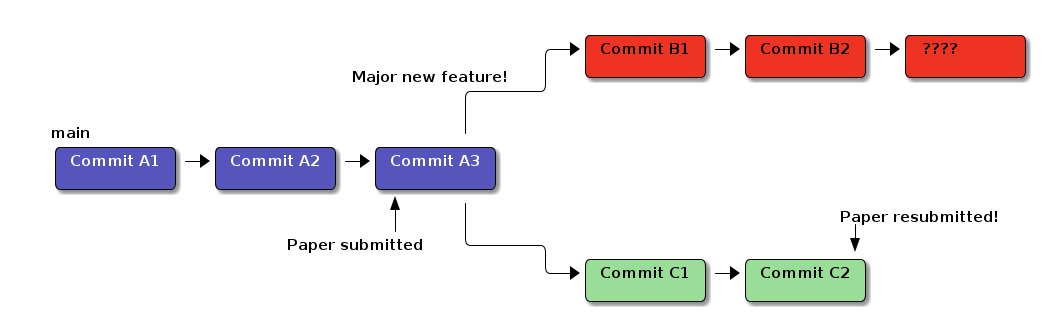
\includegraphics[scale=0.3]{figures/main_branch_040.png}
\label{branching_40_referee_changes}
\end{center}
\end{frame}
\begin{frame}[label={sec:org03792d7}]{Branching Example: Paper Accepted}
\begin{center}
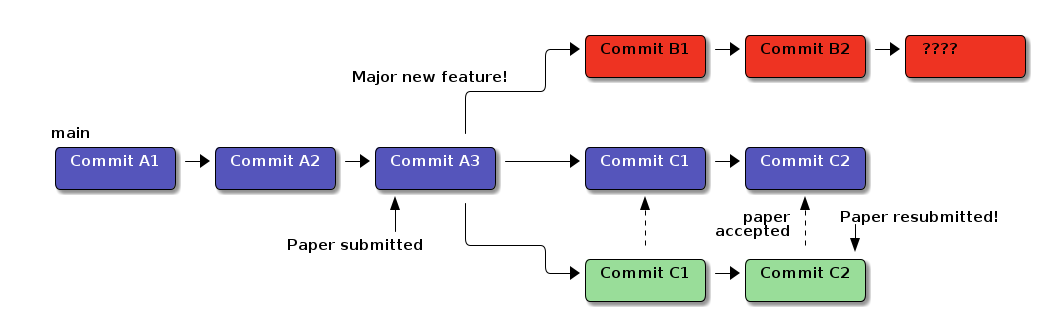
\includegraphics[scale=0.3]{figures/main_branch_050.png}
\label{branching_50_paper_accepted}
\end{center}
\end{frame}
\begin{frame}[label={sec:org30529c3}]{Branching Example: Feature Complete}
\begin{center}
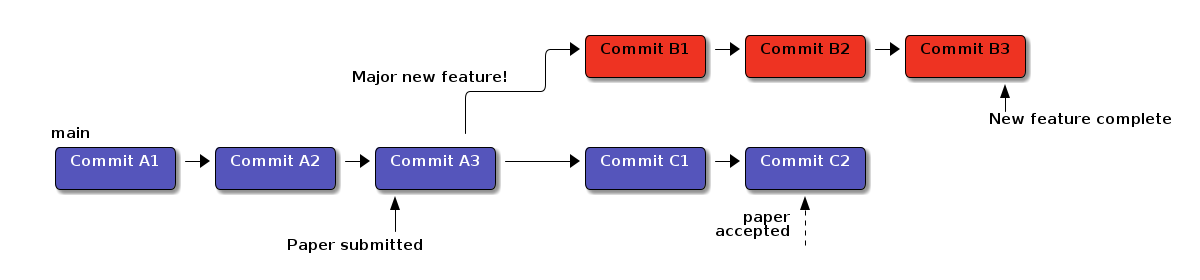
\includegraphics[scale=0.3]{figures/main_branch_060.png}
\label{branching_60_feature_complete}
\end{center}
\end{frame}
\begin{frame}[label={sec:orgd3055bc}]{Branching Example: Merge}
\begin{center}
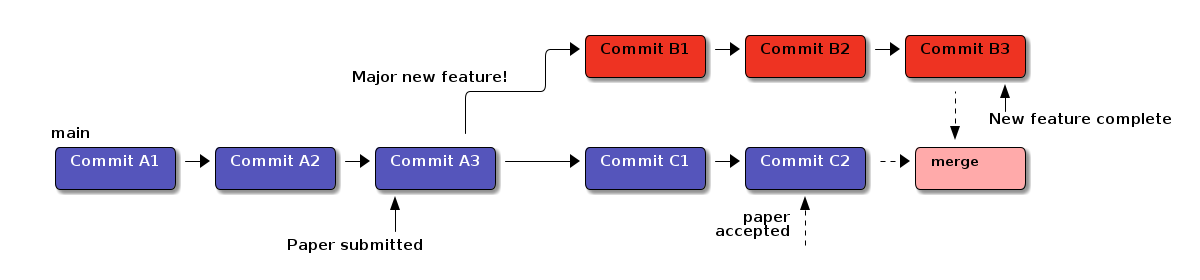
\includegraphics[scale=0.3]{figures/main_branch_070.png}
\label{branching_70_merge}
\end{center}
\end{frame}
\begin{frame}[label={sec:org162a6bd}]{Distributed Git}
You might be working at
\begin{itemize}
\item a desktop computer
\item and on a laptop
\item you might have a workstation available somewhere
\item or the HPC?
\end{itemize}

And this is all just you, a single person.

Additionally, of course: Collaborate with others!
\begin{itemize}
\item Use a server to act as a central point
\item E.g. \url{https://github.com} or \url{https://gitlab.com}
(the latter can also be hosted for free)
\end{itemize}
\end{frame}
\begin{frame}[label={sec:org618c8b0}]{Introduction to Git}
Browse to
\begin{itemize}
\item the moodle page
\url{https://moodle.nottingham.ac.uk/course/view.php?id=150881}
\item Go to \alert{Self-directed Learning Tasks}, will redirect you here:
\url{https://github.com/ricma/rse\_syllabus\_git/blob/main/content/tasks\_baking\_recipes/README.org}
\begin{center}

\includegraphics[width=0.3\columnwidth]{./figures/qr_sdlts.png}
\label{}
\end{center}
\end{itemize}
\end{frame}
\begin{frame}[label={sec:org9a13fb0},fragile]{Exercise 2 - Handling a Conflict in Real Code}
 Choose your language
\begin{description}
\item[{Python}] \url{https://github.com/RichGraham/radius\_python}
\item[{Fortran}] \url{https://github.com/RichGraham/radius\_fortran}
\item[{C / C++}] \url{https://github.com/RichGraham/radius\_c}
\item[{Matlab}] \url{https://github.com/RichGraham/radius\_matlab}
\item[{R}] \url{https://github.com/RichGraham/radius\_r}
\end{description}

Download the repository above
\begin{minted}[]{shell}
   git clone https://github.com/RichGraham/radius_<YOUR LANGUAGE>
\end{minted}

\begin{itemize}
\item Read the file \texttt{README.md} (visiting the url in a browser gives nice formatting)
\item Explore the code and changes in each branch. Make sure you can
run the code in each branch
\item \alert{Merge} the changes in \texttt{better-powers} and \texttt{proper-sqrt} as directed in the
\texttt{README.md}. Make sure the merged code runs as expected.
\end{itemize}
\end{frame}
\end{document}
